\documentclass[xcolor=pdftex,dvipsnames,table]{beamer}
%\usepackage{subfigure}
\usepackage{amsbsy}
\usepackage{tikz}
\usetikzlibrary{arrows}
\usepackage{amsmath,graphicx,dsfont,color}
\usepackage{amsfonts}
\usepackage{amssymb}
\usepackage{array}

\usepackage{subfig}

% makes the subfig package work
\makeatletter
\let\@@magyar@captionfix\relax
\makeatother

% subfigure counter resets every frame
\makeatletter
\@addtoreset{subfigure}{framenumber}
\makeatother

% First author and year
\bibliographystyle{apalike}

% This sets the list items of the bibliography to the same symbol used for citation.
\setbeamertemplate{bibliography item}{\insertbiblabel}

% This avoids extralines for different entries
\setbeamertemplate{bibliography entry title}{}
\setbeamertemplate{bibliography entry location}{}
\setbeamertemplate{bibliography entry note}{}

\DeclareMathOperator*{\argmin}{arg\,min}
\DeclareMathOperator*{\argmax}{arg\,max}
%Definitiona

\newcommand{\x}{\mathbf{x}}
\newcommand{\X}{\mathbf{X}}
\newcommand{\W}{\mathbf{W}} %Weight
\newcommand{\bais}{\mathbf{b}}%Bais
\newcommand{\act}{\texttt{g}}%Activation
\newcommand{\loss}{L}
\newcommand{\pdata}{\hat{p}_{\texttt{data}}}
\newcommand{\nsize}{N}
\newcommand{\nfeatures}{P}
\newcommand{\param}{\boldsymbol{\theta}}
\newcommand{\featmap}{\boldsymbol{\phi}}
\newcommand{\EV}{\mathbb{E}}









\title{Deep Learning for Image Analysis - Introduction}
\author{Thomas Walter, PhD}
\date{Centre for Computational Biology (CBIO) \\
	  MINES Paris-Tech, PSL Research University \\
	  Institut Curie, PSL Research University \\
	  INSERM U900}


%To include LOGO?
%\logo{\includegraphics[width=.1\columnwidth]{MinesLogo}}
\useinnertheme{rounded}
\usecolortheme{rose}

\usepackage{xcolor}
\definecolor{lightblue}{RGB}{0,200,255}

\setbeamertemplate{footline}[frame number]{}
\setbeamertemplate{navigation symbols}{}
\setbeamertemplate{section in toc}[square]
\setbeamertemplate{items}[square]


\begin{document}

\begin{frame}
\titlepage
\end{frame}

\begin{frame}{Overview}
\tableofcontents
\end{frame}

%%%%%%%%%%%%%%%%%%%%%%%%%%%%%%%%%%%%%%%%%%%%%%%%%%%%%%%%%%%%%%%%%%%%%%%%%
%%%%%%%%%%%%%%%%%%%%%%%%%%%%%%%%%%%%%%%%%%%%%%%%%%%%%%%%%%%%%%%%%%%%%%%%%
\section{Introduction: Artificial Intelligence and Machine Learning}
\frame{\frametitle{Overview}\tableofcontents[currentsection]}

\begin{frame}{Definition of Artificial Intelligence}
%\begin{definition}
%	Artificial intelligence (AI) is intelligence demonstrated by machines, in contrast to the natural intelligence displayed by humans and other animals.
%\end{definition}
\begin{itemize}
	\item The definition of the term "intelligence" is highly controversial. Usually, one understands by intelligence the capacity of an individual to reason logically, to understand complexity, to learn more or less abstract concepts, to plan and to solve problems in varying conditions. 	
	\item Artificial intelligence (AI) is intelligence demonstrated by machines, in contrast to the natural intelligence displayed by humans and other animals. 
	\item In 1956, AI became a field of research. AI can be broken down into many subfields: knowledge representation, planning, natural language processing, object manipulation (robotics), $\ldots$
\end{itemize}
\end{frame}

\begin{frame}{Definition of Machine Learning}
\begin{itemize}
	\item Machine Learning is concerned with the technology that enables computer programs to improve their performance at a certain task by experience. 
	\item In \textbf{supervised learning}, this experience comes in form of a \textbf{training set} of annotated samples, i.e. a set of observations $x_i$ together with their annotation $y_i$.
	\item In \textbf{unsupervised learning}, there are no annotations, i.e. no value of $y_i$ is given. We aim at finding \textbf{patterns} in the data that play the role of “output variables” (clusters, latent variables, …)
\end{itemize}
\end{frame}

%%%%%%%%%%%%%%%%%%%%%%%%%%%%%%%%%%%%%%%%%%%%%%%%%%%%%%%%%%%%%%%%%%%%%%%%%
%%%%%%%%%%%%%%%%%%%%%%%%%%%%%%%%%%%%%%%%%%%%%%%%%%%%%%%%%%%%%%%%%%%%%%%%%
\section{Design Principles of Machine Learning algorithms}
\frame{\frametitle{Overview}\tableofcontents[currentsection]}

\begin{frame}{A simple example: polynomial curve fitting\footnote{Example adapted from \cite{Bishop2006}}}
\begin{figure}[htb]
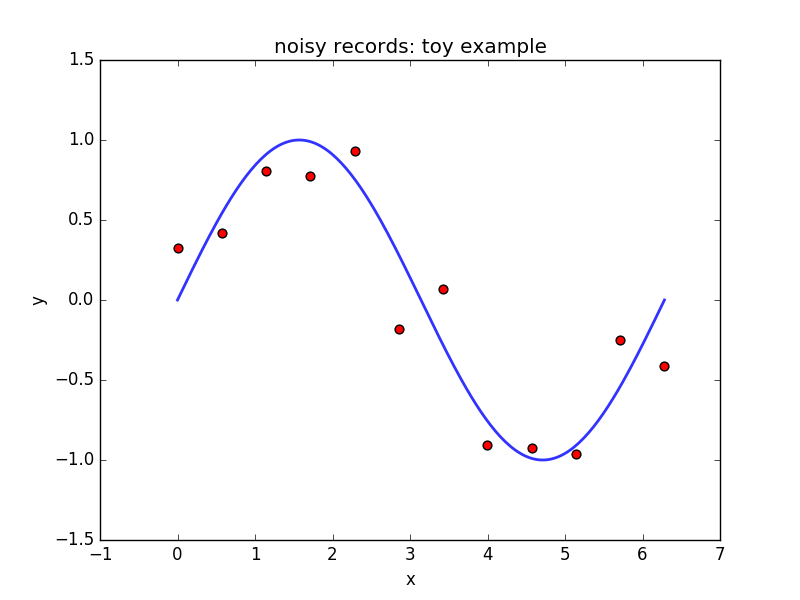
\includegraphics[width=0.6\textwidth]{../graphics/sample_from_sin.png}
\end{figure}
\begin{itemize}
	\item From a set of measured points $(x_i, y_i)$ (red), we would like to build a model to predict the value $y$ for any given $x$. 
	\item The true function is $g(x)=\sin (x)$ (displayed in blue).
	\item The measurements $y_i$ are noisy outputs of that function, i.e. 
	\begin{equation}
	y_i = \sin (x_i) + \epsilon \; , \;\;\; \;\;\; \epsilon \sim \mathcal{N}(0,0.2)
	\end{equation}
\end{itemize}
\end{frame}

\begin{frame}{A simple example: polynomial curve fitting}
\begin{itemize}
	\item We use the following polynomial model:
	\begin{eqnarray}
	f(x) &=& a_0 + a_1 x + a_2 x^2 + \ldots + a_m x^m \nonumber \\
	&=& \param^T \featmap (x)
	\end{eqnarray}
	\item Parameter vector: $\param = (a_0, a_1, \ldots, a_m)^T$
	\item Here, we do not only use the measurement $x$. We actually map $x$ to a higher dimensional space:
	\begin{eqnarray}
		\featmap : \mathbb{R}^P &\rightarrow & \mathbb{R}^Q \nonumber \\
		x &\rightarrow & \featmap (x) = (1, x, x^2, \ldots, x^m)^T
	\end{eqnarray}
	\item The model is linear in the parameters (but for $m>1$ not in the inputs). 
\end{itemize}
\end{frame}

\begin{frame}{A simple example: polynomial curve fitting}
\begin{itemize}
	\item One classical approach is to minimize the least squared error between measured and predicted values:
	\begin{eqnarray}
		\min_{\param} \loss(\param) &=& \min_{\param} \sum_{i=1}^N (y_i - f(x_i))^2 \nonumber \\
		&=& \min_{\param} \sum_{i=1}^N (y_i - \param^T \featmap (x_i))^2 
	\end{eqnarray}
	\item This can be achieved by setting the gradient with respect to $\param$ to zero:
	\begin{equation}
		\nabla_{\param} \loss = (\frac{\partial \loss}{\partial a_0}, \frac{\partial \loss}{\partial a_1}, \ldots, \frac{\partial \loss}{\partial a_m} )^T = 0
	\end{equation}
	\item Unlike for most optimization problems in this course, this leads to an analytical solution for $\param$. This is known as \textbf{linear regression}. For more details, we refer to \cite{Hastie2009}.
\end{itemize}
\end{frame}

\begin{frame}{Overfitting and underfitting}
\begin{figure}[htb]
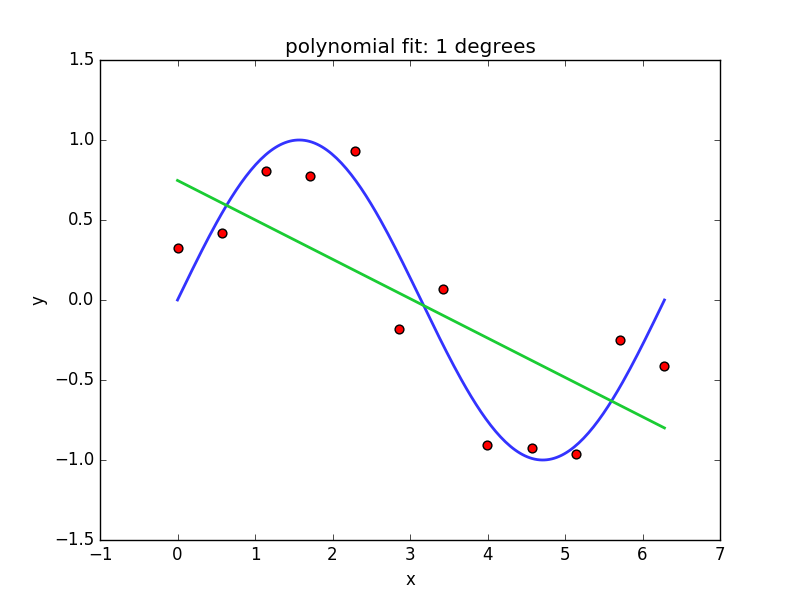
\includegraphics[width=0.6\textwidth]{../graphics/polyfit_degree_1.png}
\end{figure}
For $m=1$, the model is linear in its inputs. The solution is not capable of modeling the measured data points; we get a poor approximation of the original function. The family of functions we have used was not complex enough to model the true data distribution. We also speak of \textbf{underfitting}.
\end{frame}

\begin{frame}{Overfitting and underfitting}
\begin{figure}[htb]
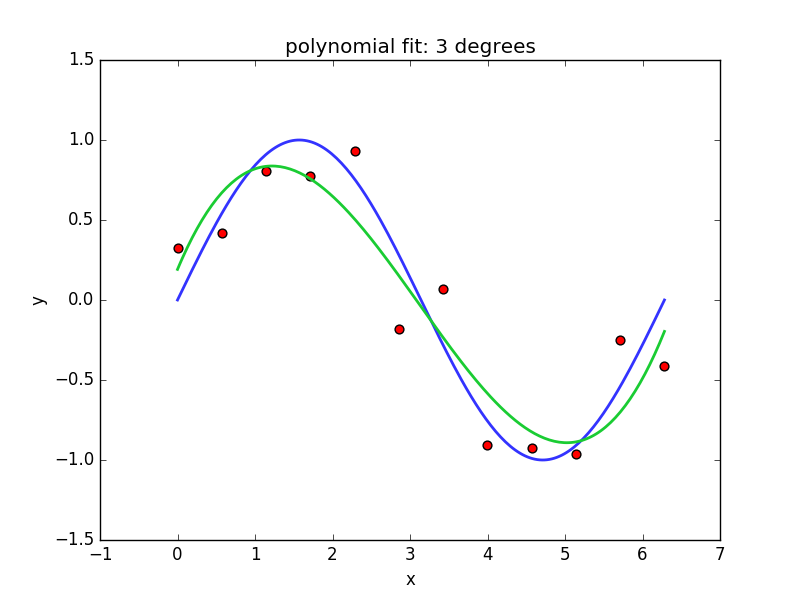
\includegraphics[width=0.6\textwidth]{../graphics/polyfit_degree_3.png}
\end{figure}
For $m=3$, we obtain a solution that seems to be quite right: it is sufficiently complex to model the true data distribution, but not too complex to model the small variations which are due to noise.
\end{frame}

\begin{frame}{Overfitting and underfitting}
\begin{figure}[htb]
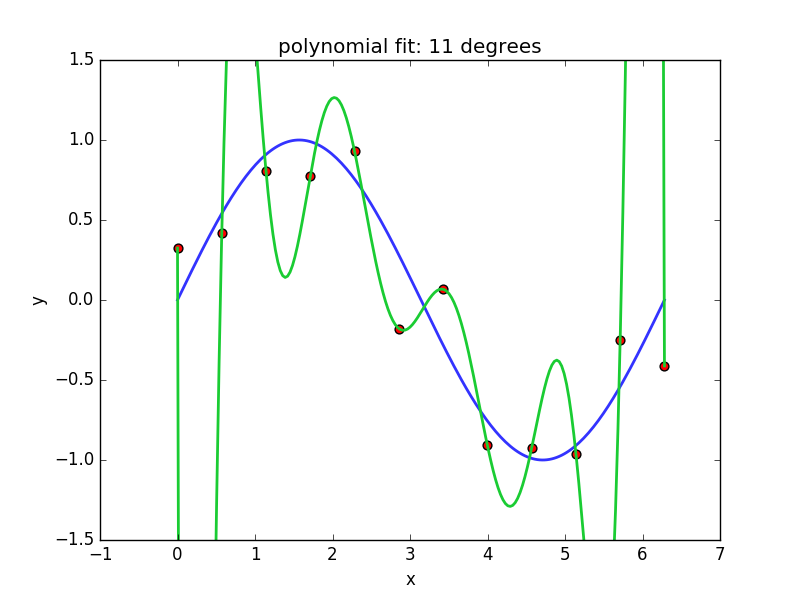
\includegraphics[width=0.6\textwidth]{../graphics/polyfit_degree_11.png}
\end{figure}
For $m=11$, we obtain a solution that has zero error (the function passes through every point of the training set). But the coefficients with large absolute values that cancel each other precisely on the training points lead to a highly unstable function. We speak of \textbf{overfitting} and \textbf{poor generalization}.
\end{frame}

\begin{frame}{Overfitting and underfitting}
\begin{figure}[htb]
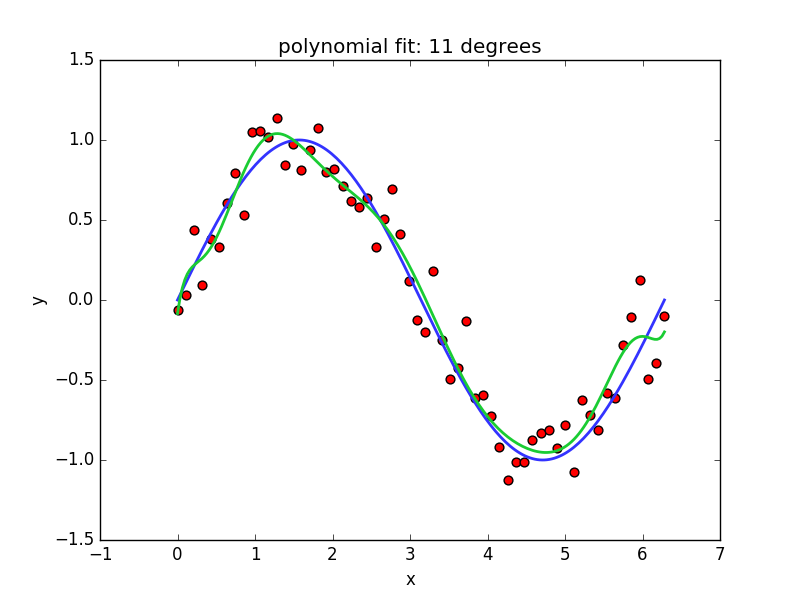
\includegraphics[width=0.6\textwidth]{../graphics/polyfit_degree_11_N60.png}
\end{figure}
One way of reducing overfitting is to increase the number of samples. Even if the function is complex, it cannot be “too wild”, as it has to find a compromise between many training samples. This however implies the annotation (or measurement) of more samples. 
\end{frame}

\begin{frame}{Overfitting and underfitting}
\begin{figure}[htb]
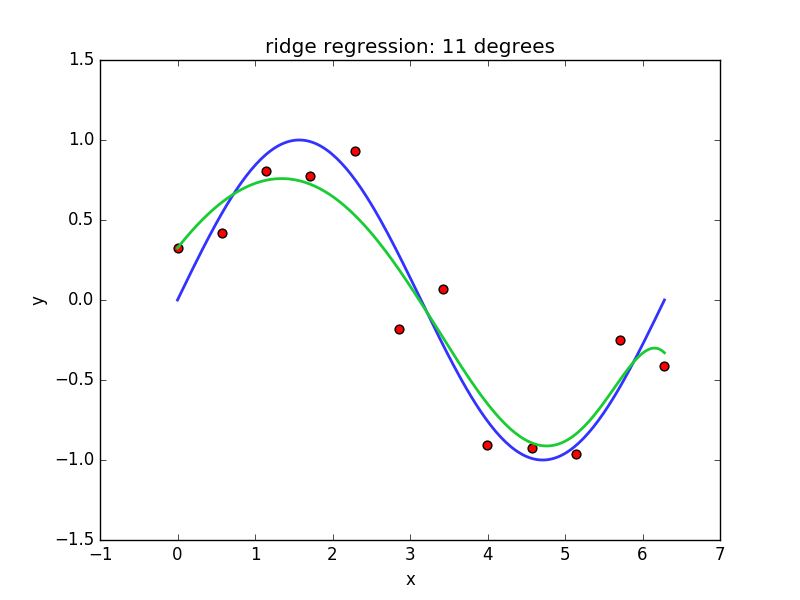
\includegraphics[width=0.6\textwidth]{../graphics/ridge_regression_11_10.png}
\end{figure}
Another way of preventing overfitting without increasing the number of samples, is to add a penalization term in the optimization procedure. This is also known as \textbf{regularization}:
\begin{equation}
	\loss = \sum_{i=1}^N (y_i - \param^T \featmap (x_i))^2 + \lambda \| \param \|^2
\end{equation}
\end{frame}


%%%%%%%%%%%%%%%%%%%%%%%%%%%%%%%%%%%%%%%%%%%%%%%%%%%%%%%%%%%%%%%%%%%%%%%%%
%%%%%%%%%%%%%%%%%%%%%%%%%%%%%%%%%%%%%%%%%%%%%%%%%%%%%%%%%%%%%%%%%%%%%%%%%
\section{Supervised Learning: Example algorithms}
\subsection{Nearest Neighbor classification}
\subsection{Random Forests}
\subsection{Linear Discriminant Analysis (LDA)}
\subsection{Support Vector Machines (SVM) and kernel methods}

%%%%%%%%%%%%%%%%%%%%%%%%%%%%%%%%%%%%%%%%%%%%%%%%%%%%%%%%%%%%%%%%%%%%%%%%%
%%%%%%%%%%%%%%%%%%%%%%%%%%%%%%%%%%%%%%%%%%%%%%%%%%%%%%%%%%%%%%%%%%%%%%%%%
\section{References}
\begin{frame}[allowframebreaks]
	\frametitle{References}
	\bibliography{slides_deep.bib}
\end{frame}


\end{document}